\section{Introduction}
\label{sec:intro}
Loading and storing information to memory is an intrinsic part of any computer program. As illustrated in Figure~\ref{fig:cpuvsmemory}, the past few decades have seen the performance gap between processors and memory grow. Even with the saturation and demise of Moore's law~\cite{Wulf1995, waldrop2016, MooreMITR}, processing power is expected to grow as multi-core architectures become more reliable~\cite{Geer}. The end-to-end performance of a program heavily depends on both processor and memory performance. Slower memory systems can bottleneck computational performance. This has been driving motivation for computer architects and researchers to explore strategies for shortening memory access latency, including sustained efforts towards enhancing the memory hierarchy~\cite{Burger}. Despite these efforts, long-latency memory accesses do occur when there is a miss in the last level cache (LLC). This triggers an access to shared memory, and the processer is stalled as it waits for the shared memory to return the requested information. 

%---------------------------
\begin{figure}[t!]
\centering
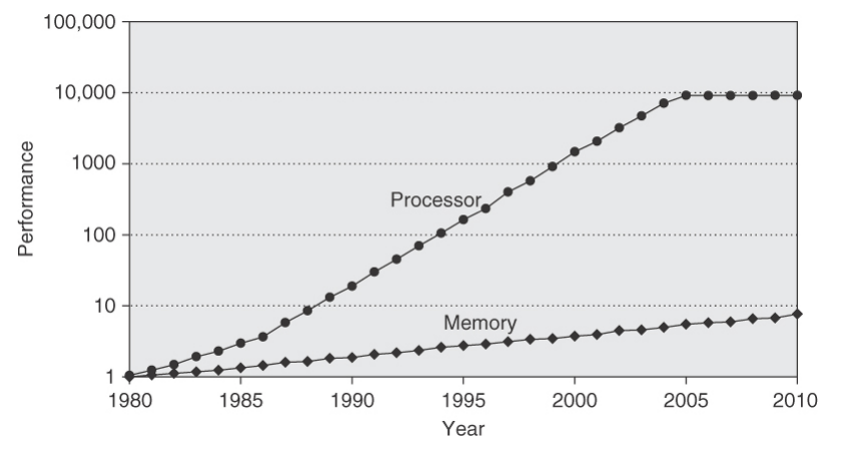
\includegraphics[width=0.7\linewidth]{fig/cpuvsmemory.jpg}
\caption{\it{The gap in performance, measured as the difference in the time 
between processor memory requests (for a single processor or core) and the 
latency of a DRAM access, is plotted over a $30$ year span~\cite{comparchbook}.}}
\label{fig:cpuvsmemory}
\end{figure}
%---------------------------
In multi-core systems, shared memory access conflicts between cores result in large access request queues. Figure~\ref{fig:multicore_arch}  illustrates a general multi-core architecture. The bank queues are served every memory clock cycle and the acknowledgement with data is sent back to the corresponding processor. In scenarios where multiple cores request access to memory locations in the same bank, the memory controller arbitrates them using bank queues. This contention between cores to access from the same bank is known as a {\em bank conflict}. As the number of bank conflicts increases, the resultant increases in memory access latency causes the multi-core system to slow.

%---------------------------
\begin{figure}[t!]
\centering
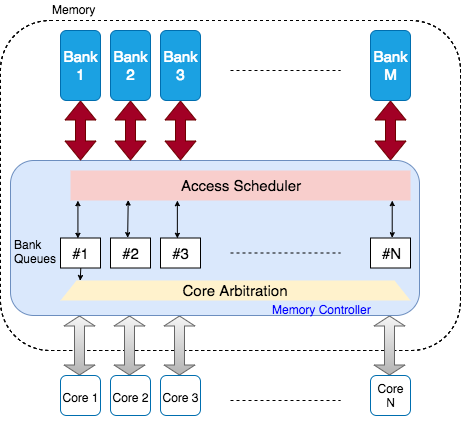
\includegraphics[width=\linewidth]{fig/fig-2-memory-controller.png}
\caption{\it{General multi-core architecture with a shared memory. $N$ processor cores share a memory consisting of $M$ banks.}}
\label{fig:multicore_arch}
\end{figure}
%---------------------------
We address the issue of increased latency by introducing a coded memory design. The main principle behind our memory design is to distribute accesses intended for a particular bank across multiple banks. We redundantly store encoded data, and we decode memory for highly requested memory banks using idle memory banks. This approach allows us to simultaneously serve multiple read requests intended for a particular bank. Figure~\ref{fig:example_xor} shows this with an example. Here, Bank 3 is redundant as its content is a function of the content stored on Banks 1 and 2. Such redundant banks are also referred to as {\em parity banks}. Assume that the information is arranged in $L$ rows in two first two banks, represented by $[a(1),\ldots, a(L)]$ and $[b(1),\ldots, b(L)]$, respectively. Let $+$ denote the XOR operation, and additionally assume that the memory controller is capable of performing simple decoding operations, \textit{i.e.} recovering $a(j)$ from $b(j)$ and $a(j) + b(j)$. Because the third bank store $L$ rows containing $[a(1) + b(1),\ldots, a(L) + b(L)]$, this design allows us to simultaneously serve any two read requests in a single memory clock cycle.   

%---------------------------
\begin{figure}[t!]
\centering
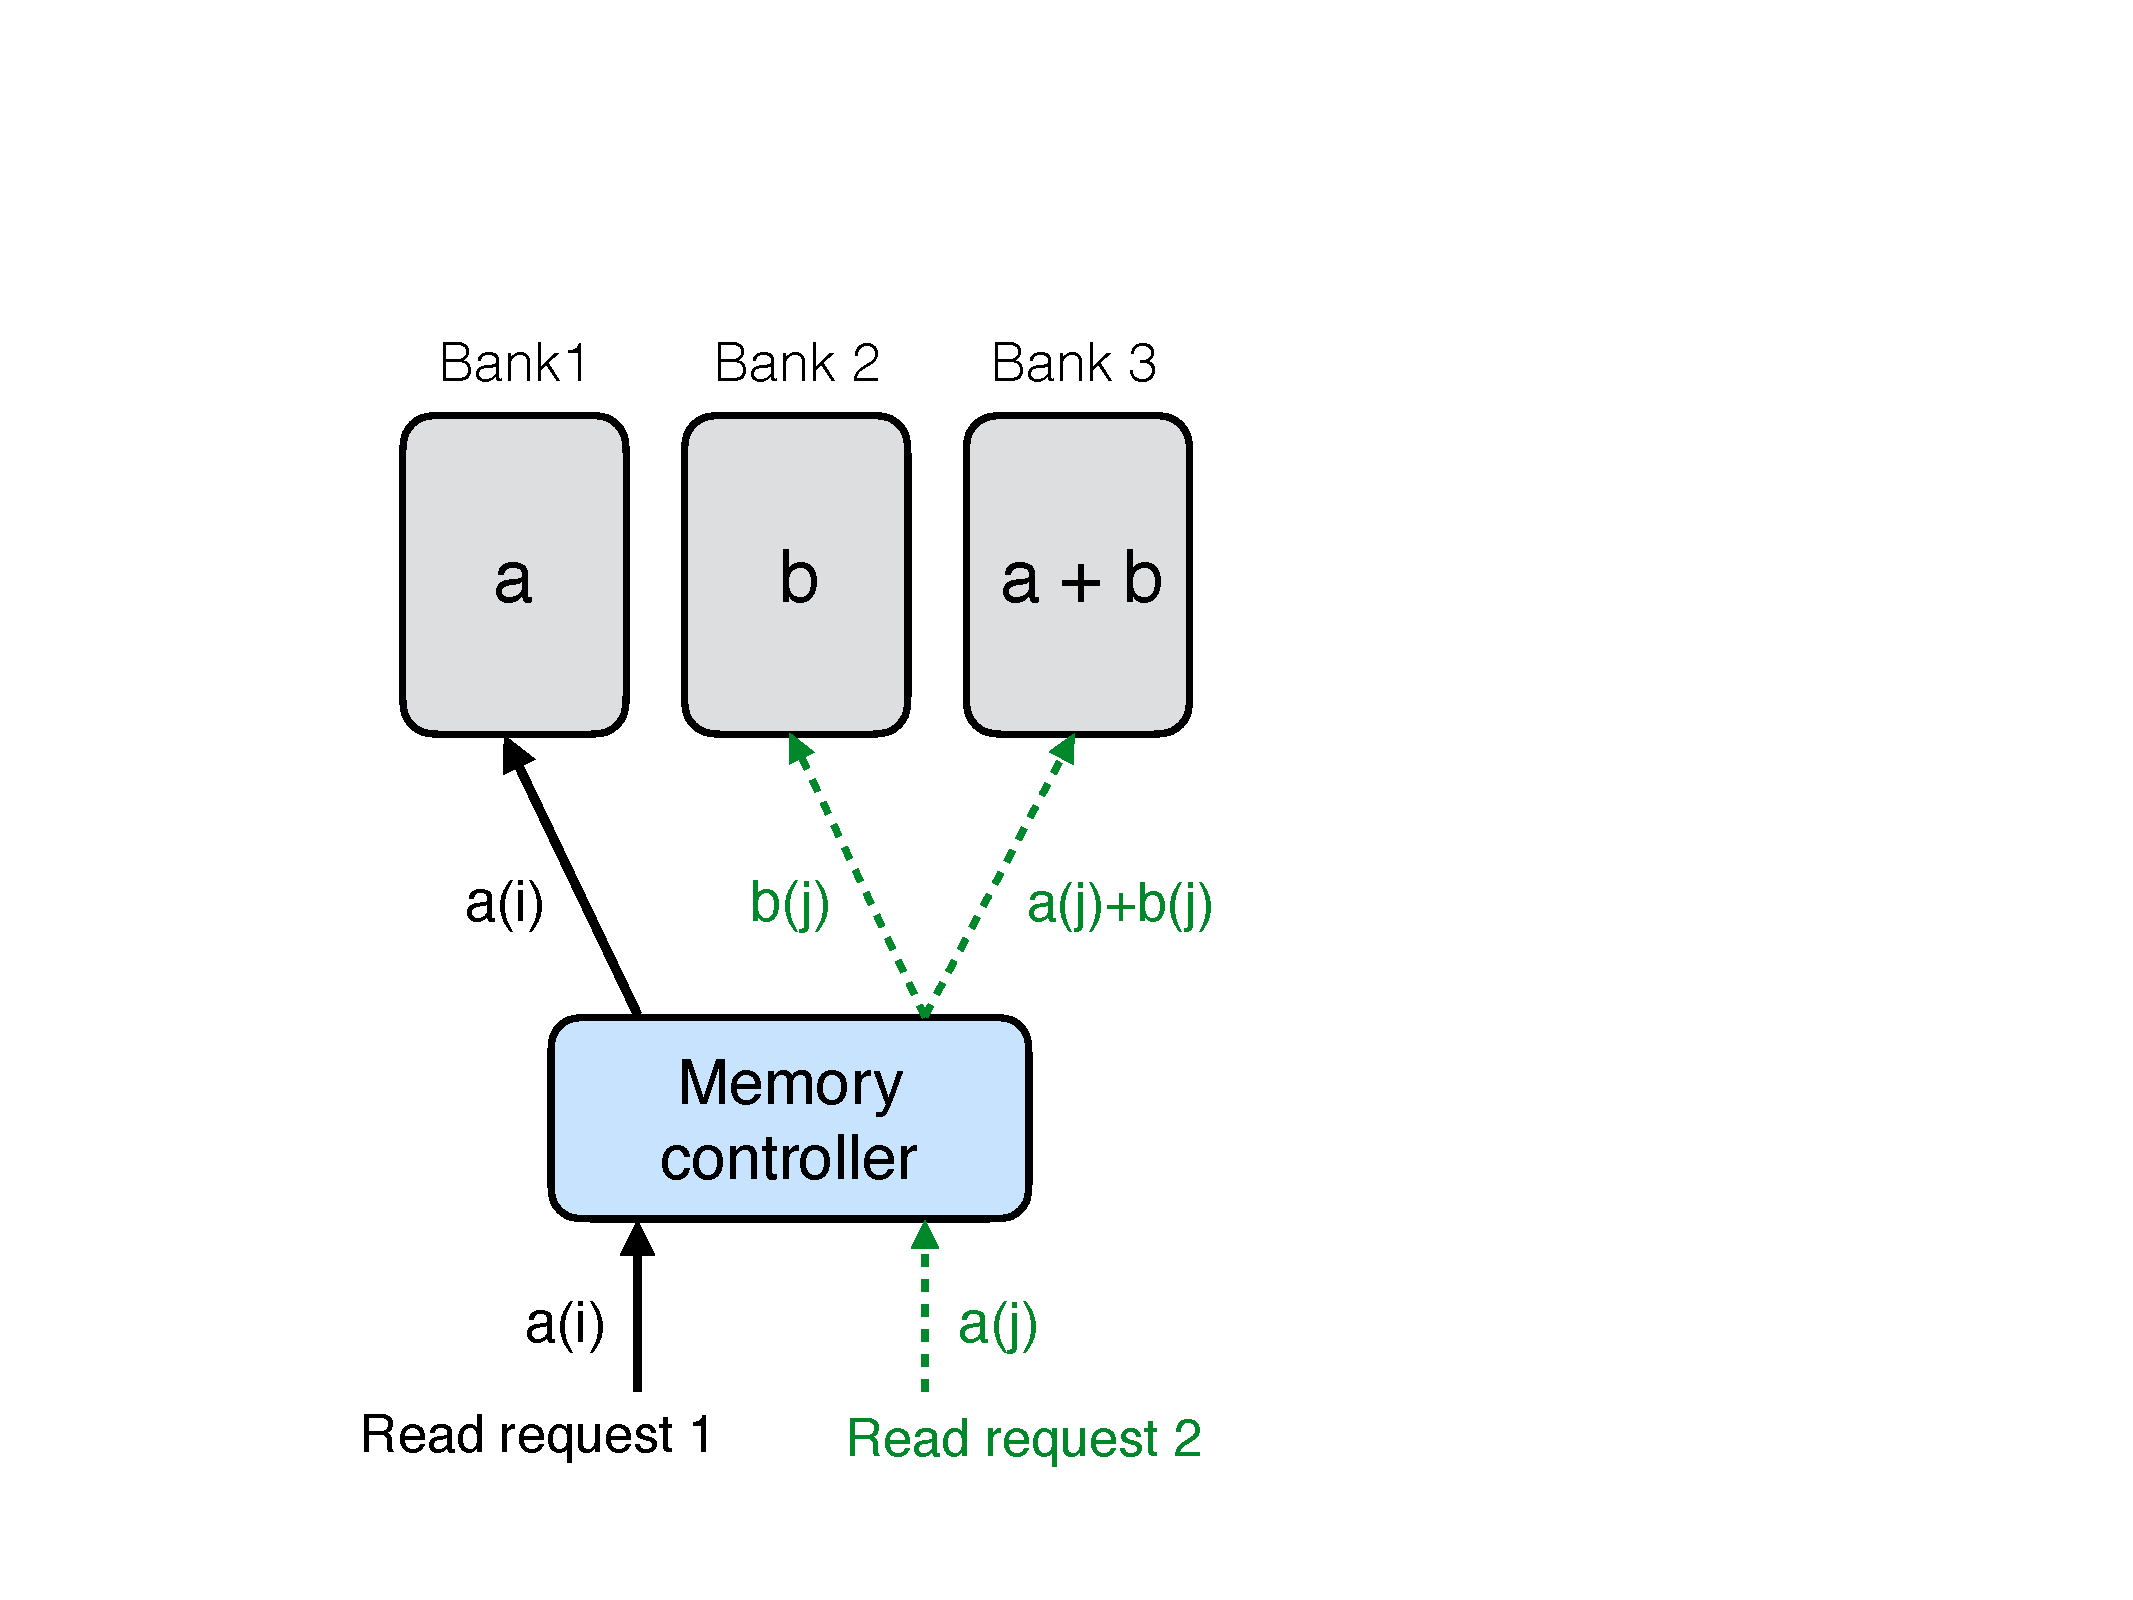
\includegraphics[width=0.395\linewidth]{fig/example-xor.pdf}
\caption{\it{Enabling multiple read accesses to a bank by coding. Given two read requests $\{a(i), a(j)\}$ directed to Bank $1$, we can deal with bank conflict in the following manner: 1) First request for $a(i)$ can be directly served by Bank $1$ itself, and 2) The read request for $a(j)$ can be served by downloading $b(j)$ and $a(j) + b(j)$ from Bank 2 and Bank 3, respectively. Another case where two read request corresponding to two different banks, e.g., $\{a(i), b(j)\}$, can be simultaneously served from their respective banks without utilizing Bank $3$.}}
\label{fig:example_xor}
\end{figure}
%---------------------------
On top of serving read requests more robustly, hybrid memory designs such as the one in Figure~\ref{fig:example_xor} have additional requirements on top of serving read requests. The presence of redundent parity banks raises a number of challenges while serving write requests. The memory overhead of redundent memory storage adds to the overall cost of such systems, so efforts must be made to minimize this overhead. Finally, the heavy memory access request rate possible in multi-core scenarios necessitates sophisticated scheduling strategies which are performed by the memory controller. In this paper we address these design challenges and evaluate potential solutions in a simulated memory enviornment. 

\noindent \textbf{Main contributions and organization:~}In this paper we systematically address all key issues pertaining to a shared memory system that can simultaneously service multiple access requests in a multi-core setup. We present all the necessary background on realization of multi-port memories using single-port memory banks along with an account of relevant prior work in Section~\ref{sec:bg}. We then present the main contributions of the paper which we summarize below. %Here, we highlight the main contributions of the paper. 
\begin{itemize}
\item We focus on the design of the storage space (array of memory banks) in Section~\ref{sec:code_design}. In particular, we employ three specific coding schemes to redundantly store the information in memory banks. These coding schemes, which are based on the literature on distributed storage systems~\cite{dimakis, Gopalan12, batchcodes, RPDV16}, allow us to realize the functionality of multi-port memories from a single port memories while efficiently utilizing the storage space. Moreover, these coding schemes have low complexity encoding and decoding processes that require only simple XOR operation. %We focus on two specific memory designs that store information in memory banks based on two different coding schemes from the literature on distributed storage systems (a.k.a. cloud storage systems)~\cite{dimakis, Gopalan12, batchcodes, RPDV16}. These coding schemes allow us to realize the functionality of multi-port memories from a single port memories while efficiently utilizing the storage space. Moreover, these coding schemes have low complexity encoding and decoding processes that require only simple XOR operation.
\item We present a memory controller architecture for the proposed coding based memory system in Section~\ref{sec:memcontrol}. Among other issues, the memory controller design involves devising scheduling schemes for both read and write requests. This includes careful utilization of the redundancy present in the memory banks while maintaining the validity of information stored in them.
%In our setup, these scheduling schemes need to take the underlying coding scheme into account in order to utilize the redundancy present in the array of memory banks in the best possible manner. Furthermore, we also address the issue of keeping track of the validity of the information stored in various banks. Note that, due to unserved previous write requests, some of the stored data might have become outdate as far as a particular read request is concerned.
%able to serve the masecond main component of a shared memory system, i.e., memory controller, in Section~\ref{sec:memcontrol}. The memory controller design We also design the memory controllers for the proposed memory systems based on the storage pattern in different memory banks. Note that the memory controller design involves devising buffering and arbitration (scheduling) schemes for both read and write requests.
\item Focusing on applications where memory traces might exhibit favorable access patterns, we explore two ways to improve the efficiency of our coding based memory design in Sections~\ref{sec:dynamicCoding} and~\ref{sec:prefetching}. First, we propose a dynamic coding scheme which is based on continuous detection of heavily accessed regions on memory banks. 
%The dynamic coding scheme only encode these heavily access regions at a particular time instance. As different (uncoded) regions begin receiving more accesses, the dynamic coding scheme updates the content of parity (redundant) memory banks by encoding these regions. 
The second solution involves predicting the patterns of memory addresses in different access requests. 
%Based on this prediction, the data from free bank is prefetched to serve subsequent request for information with the help of the prefetched data. This creates the opportunities to serve a large number of access requests in a given memory clock cycle. We note that the design of such prefacing schemes crucially depends on the underlying coding scheme.
%with Accompanied the design using dynamic coding where data is moved between coded and uncoded states. Utilized the coded memory system to perform useful data prefetching.
\item {\color{blue}Finally, we conduct a detailed evaluation of the proposed designs of shared memory systems in Section~\ref{sec:simulation}. We implement our memory designs using system C and evaluation the overall performance of these designs by regressing their system C implementation through memory traces from real multi-core systems. In addition, we also analyze the performance of our purposed designs with the help of extensive simulation on Ramulator, a DRAM simulator designed by Kim et al.~\cite{Ramulator}.} %a Implementation of the proposed solution using system C. Performance evaluation of the proposed solution on real memory traces with the help the system C implementation.  evaluate each
%of them for their cost. We also implement these designs using systemC and regress it throughmemory traces from real multi-core system.
\end{itemize}

%problem of concentrated accesses to a particular bank by normalizing it across 
%several banks. The solution is to use coding theory techniques to create 
%redundancy across banks, increasing the number of parallel accesses per cycle.  
%The queue build up on a bank is serviced through parallel access to several 
%additional banks, known as parity banks. The additional bank accesses results in 
%a decrease in number of contended memory accesses between cores, therefore 
%reducing the overall latency of the system. The reduction in the latency can be 
%seen directly as an increase in the overall system performance. 
%We present various design to store the redundancy across the parity banks and evaluate each
%of them for their cost. We also implement these designs using systemC and regress it through
%memory traces from real multi-core system.
%We show that 
%with a memory overhead of 15 $\%$; we can enable 4 extra read accesses / 2 extra 
%write accesses to a bank while remaining within the given design parameters. 

%{\color{blue}
%\subsection{Main contributions}
%
%Here, we summarize the main contributions of this paper. 
%\begin{itemize}
%\item Taking a coding theoretic approach to address the issue of realizing multi-port memories from single port memories. 
%\item Designed the memory controller accordingly:
%\begin{itemize}
%\item Involves devising scheduling schemes for both read and write requests.
%\end{itemize}
%\item Accompanied the design using dynamic coding where data is moved between coded and uncoded states. 
%\item Utilized the coded memory system to perform useful data prefetching.
%\item Implementation of the proposed solution using system C. Performance evaluation of the proposed solution on real memory traces with the help the system C implementation. 
%\end{itemize}
%}

%\noindent \textbf{Organization:~} The rest of the paper is organized as follows.

%\textbf{Key issues that need to be addressed}

%\begin{itemize}
%\item Design of storage space, i.e., how the data is distributed among different memory banks. This includes generation of redundancy (parity bits) based on the original data and allocation of these parity bits to the memory banks.
%\item Keeping track of the validity of the data stored in various banks. Note that, due to unserved previous write requests, some of the stored data might have become outdate as far as a particular read request is concerned.
%\item Resource allocation/arbitration among the different read and write requests originated from the same or different processors. The arbitration mechanism should take multiple criterion into account, including performance (i.e., the latency viewed by the processors), efficient utilization of the storage space (i.e., minimize the unused memory bank during a given period of time), and fairness (i.e., no processor should unnecessarily suffer due to requests from other processors getting prioritized).
%\end{itemize}

%%%%%%%%%%%%